\subsection{Data Model}
To represent a continuous function devoid of a closed-form
representation, a digital computer must store measurements of the
function at discrete samples taken in a given domain. Yet
rendering numerical data typically requires knowledge of the values
between samples to produce perceptually continuous images from
arbitrary viewpoints. To develop efficient algorithms, visualization
tools often decompose data into structure and
attributes~\cite{vtk}. Structure encapsulates both the locations and
connectivity relations onto which attributes are mapped and
connectivity information serves to constrain the interpolation
problem. Note that some authors continue the abstraction of structure
into topology and geometry~\cite{weiler}, however in the context of
this research, topology is synonymous with
structure. Figure~\ref{fig:data_hierarchy} outlines the data model
adopted by \sciwms{}. A dataset is composed of attributes with
associated structure which is further classified as a regular or
irregular, known as {\bf \cgrid{} } and {\bf \ugrid{}} topologies in
\sciwms{} documentation.
\begin{figure}[ht!]
  \centering
  \begin{subfigure}[t]{0.45\columnwidth}
    \centering
    \includegraphics[width=\columnwidth]{../figs/data_model_hierarchy}
    \caption{}
    \label{fig:data_hierarchy}
  \end{subfigure}
  \begin{subfigure}[t]{0.45\columnwidth}
    \centering
    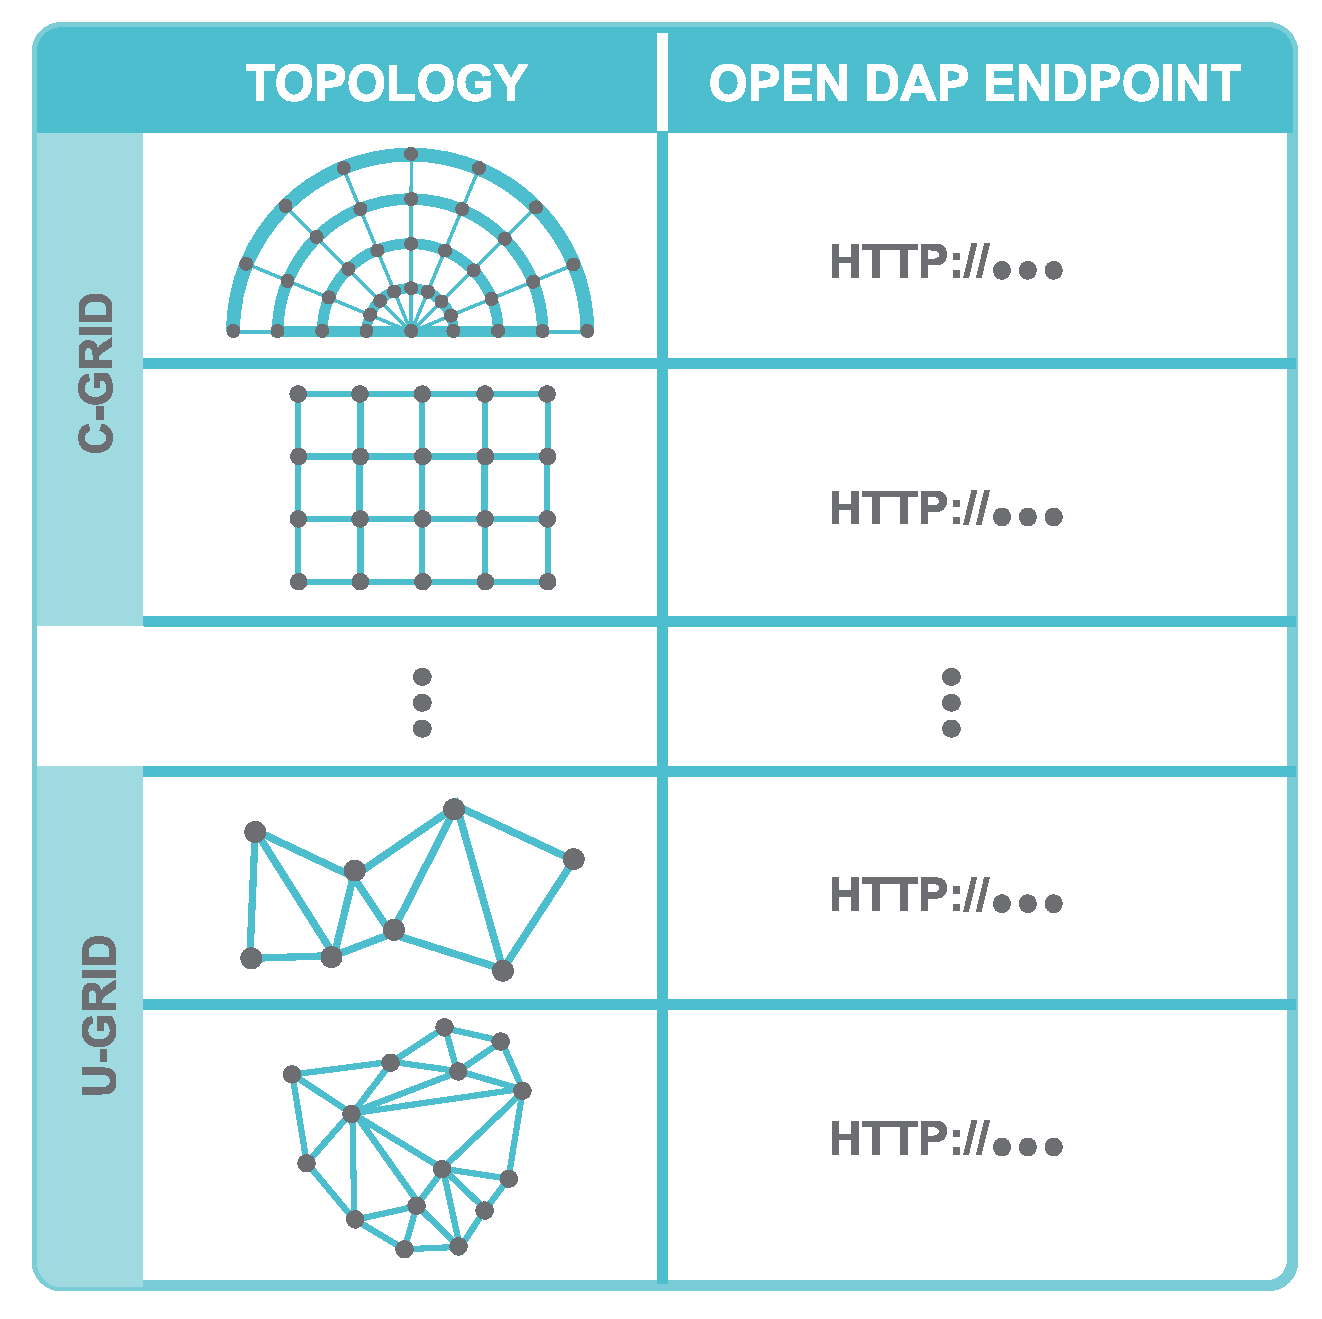
\includegraphics[width=\columnwidth]{../figs/sciwms_book_db_topology_endpoint_chart}
    \caption{}
    \label{fig:sciwms_topology_endpoints}
  \end{subfigure}
  \caption{(a) Decomposition hierarchy of the data model.  (b)
    \Sciwms{} topology and endpoint data store.}
\end{figure}
